\documentclass[class=NCU_thesis, crop=false]{standalone}
\begin{document}

\chapter{Study on the Background Estimation}
	As mentioned in the last chapter, the CRs are used to estimate the backgrounds in the SR. Because W+jets events and $t\bar{t}$ events in both SR and one-muon CR are the same processes, one assumes the kinematics are the same. As for the two-lepton CR, first note that the mass of the charged leptons and neutrinos are negligible compared to that of the Z boson. Thus, one can argue that the kinematics of the Z(ll)+jets and Z($\nu \nu$)+jets events are roughly the same, where the Z(ll) means the charged-leptonic decay of the Z boson.
	
	During the analysis, the author and Po-Shan Shih, partner of the author, are both working on the estimation of the two-lepton CR. In this chapter, the problems that the author participated or fixed during the study are stated. Also, a shape difference of W($\mu \nu$)+jets events in SR and one-muon CR is carried out as an additional work.
	
	\section{Overlap Removal}
		The comparison plots of Monte Carlo (MC) to data are always reviewed by analyzers. Those plots are referred to as the pre-fit plots. The pre-fit plots contain the data and MC samples that pass the selection criteria. Those events are then filled in the plot based on the value of the physical quantity of interest.
		
		An unusual peak was spotted in one of the Z+jets CR plot during the analysis, as shown in figure \ref{fig:OR_before}. The plot is the distribution of the leading large-R jet mass and the peak is within 90 to 105 GeV. It is unusual because the statistics of the mass spectum should generally become less as the energy goes up. However, the peak reveals that many events assemble around a high energy value and thus creates a discontinuity.
		
		\fig[0.5][fig:OR_before][!hbt]{OR_before.png}[The plot which shows the issue of overlap removal. It shows the distribution of leading large-R jet mass. The dotted points represent the data while the solid histogram shows the MC simulations. Both of them pass the selection criteria of two-lepton CR. The spotted unusual peak lies in the bin of 90 to 105 GeV. The legends of "Z+mumu" and "Z+ee" in the upper-right of the plots are typos which weren't fixed at that time. They refer to the MC simulations of Z(ee)+jets and Z($\mu \mu$)+jets events respectively.][short caption]
		
		The bin includes the Z boson mass, which is about 91 GeV. From the Feynman diagram of the Z+jets background (figure \ref{fig:subfig_Zjets}) with the neutrinos replaced with leptons, one can tell that the invariant mass of the lepton pair would be close to that of a Z boson. In figure \ref{fig:OR_before}, nevertheless, it is large-R jet that has the invariant mass around it.

		Because all these events pass the two-lepton CR selections as stated in section \ref{2LCR}, one of the possible explanation to this peak is misidentification of leptons and large-R jets. It happens when they share the same track or overlap. From figure \ref{fig:OR_before}, one recognizes that the Z(ee)+jets events contributes the most in that bin. Recall the last reconstruction strategy from section \ref{OR} that an electron is removed if it it within $\Delta R = 0.1$ with a large-R jet.
		
		As a result, a check in the codes on the overlap removal (OR) was conducted, and the same plot after adding it is shown in figure \ref{fig:OR_after}. From the plot, one can see that the peak around the Z boson mass is removed. This discovery and study reveal the fact that OR wasn't properly applied at that time. After a careful check on the codes with the developer of the framework we used, the OR problem was officailly fixed.
		
		\fig[0.5][fig:OR_after][!hbt]{OR_after.png}[The plot which shows the result after overlap removal applies properly. The dotted points represent the data while the solid histogram shows the MC simulations.][short caption]
	
	\section{Dealing with Large Weights}
		There are unexpected situation during real data collecting at the detector, which is not simulated by the MC. To further include these possibilities in the simulations, weights are applied. After the calculations done by MC, the raw number of events would be multiplied by these weights.
		
		Another peak was discovered in the Z+jets CR plot during the analysis, as shown in figure \ref{fig:unfixed posW}. The shown plot is also the distribution of leading large-R jet mass, but it also appeared in other different plots. Following the logic in the last section, one can tell that it is unusual. However, because of the fact that OR had fixed this time and also because of this spike-like behavior existed in other kinematic variable plots, it must be a result of a different issue.
		
		As it turned out, an event was multiplied by a really high generator weight which resulted in a large contribution to the MC. The reason of this is a result of a random generation, which happens in the the type of MC generator the analyzers used. Another similar weird behavior could happen when the generator weight is a great negative value, as shown in figure \ref{fig:unfixed negW}, which was another plot during the analysis. A clear pit shows up in the distribution where it should be continuous.
		
		\fig[0.6][fig:unfixed posW][!hbt]{unfixed_posW.jpg}[The plot which shows the unusual peak resulting from the generator weight. It shows the distribution of leading large-R jet mass. The dotted points represent the data while the solid histogram shows the MC simulations. The legends of "Z+mumu" and "Z+ee" in the upper-right of the plots are typos which weren't fixed at that time. They refer to the MC simulations of Z(ee)+jets and Z($\mu \mu$)+jets events respectively.][short caption]
		
		\fig[0.6][fig:fixed posW][!hbt]{fixed_posW.jpg}[The plot which shows the result after the event with large generator weight removed. Comparing to \ref{fig:unfixed posW} reveals that the peak disappears.][short caption]
		
		The solution to these weights in this iteration is to remove those events, because the number of events with these extreme value of generator weight is small and negligible. The results after removing the events are shown in figure \ref{fig:fixed posW} and \ref{fig:fixed negW}.
		
		\fig[0.6][fig:unfixed negW][!hbt]{unfixed_negW.pdf}[The plot which shows the unusual pit. It shows the distribution of dijet mass. The dotted points represent the data while the solid histogram shows the MC simulations.][short caption]
		
		\fig[0.6][fig:fixed negW][!hbt]{fixed_negW.pdf}[The plot which shows the result after the events with large negative value of generator weight are removed. Comparing to \ref{fig:unfixed negW} reveals that the pit disappears.][short caption]
	
	\section{W($\mu \nu$) +jets Events Shape Comparison}
		As mentioned in the beginning of this chapter, the W+jets and $t\bar{t}$ events in either SR or one-muon CR are assumed to have the same kinematics. Thus, one-muon CR can be made use of estimating the background in SR. However, the author wonders whether the comparison of the kinematics between these two regions matches. Therefore, a study on this is performed.
	
		A set of W($\mu \nu$)+jets Monte-Carlo (MC) samples is used. In these samples, the selection for one-muon CR and SR mentioned in the last chapter are applied. The samples after the selections of SR is used as a comparison to the one-muon CR.
		
		The reason why a comparison between W($\mu \nu$)+jets samples and data is not used is because one cannot know the truth-level comparison via it. The data after the one-muon selections would contain the $t\bar{t}$ events since they are also one of the estimation target of one-muon CR. If one adds the $t\bar{t}$ MC samples in the comparison, data and MC comparison is apple-to-apple, but one would lose the information of the shape difference on W($\mu \nu$)+jets events only. 

		Because one doesn't know the yields of both samples after the selection, a normalization is used on them. After normalization, one can deduce the shape difference without any adjustment on the yields of one of them. The events are put in a histogram plot for comparison. The shape comparison for (proxy) $E_T^{\mathrm{miss}}$ is shown in figure \ref{fig:MET_comparison}. Besides, a yields uncertainty of 5\% is assigned to this SR and one-muon CR extrapolation. The reason of 5\% is due to the fact that some uncertainties used in this analysis follow the results of another analysis group, the Vh(bb) group, including this uncertainty value.
		
		\fig[0.6][fig:MET_comparison][!hbt]{manybins.pdf}[placeholder.][short caption]

		%\begin{figure}[!hbt]
			%\captionsetup[subfigure]{labelformat=empty} % hide figure's number.
		%	\centering
		%	\subcaptionbox
		%	{\label{fig:subfig_onePTV}}
		%	{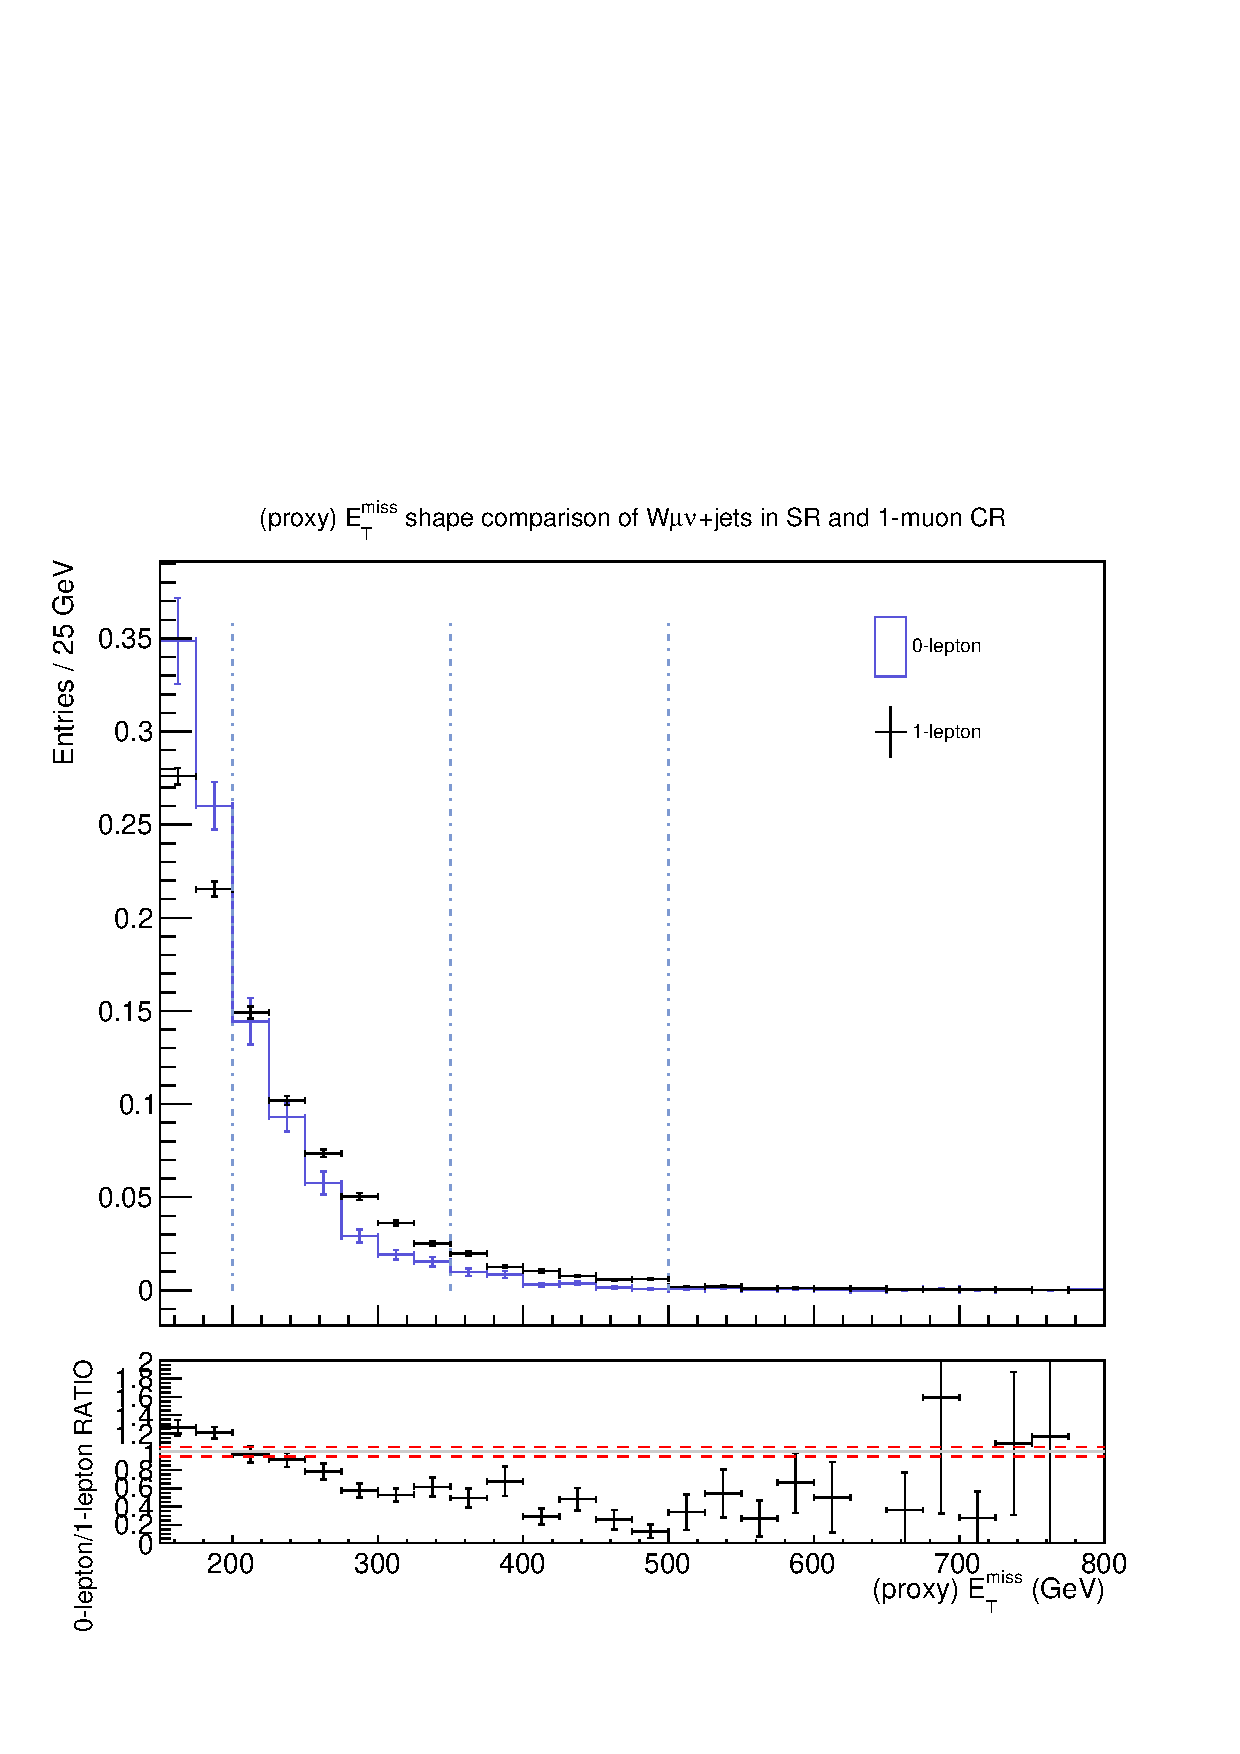
\includegraphics[width=0.45\linewidth]{manybins.pdf}}
		%	~
			%\vspace{\baselineskip}
		%	\subcaptionbox
		%	{\label{fig:subfig_twoPTV}}
		%	{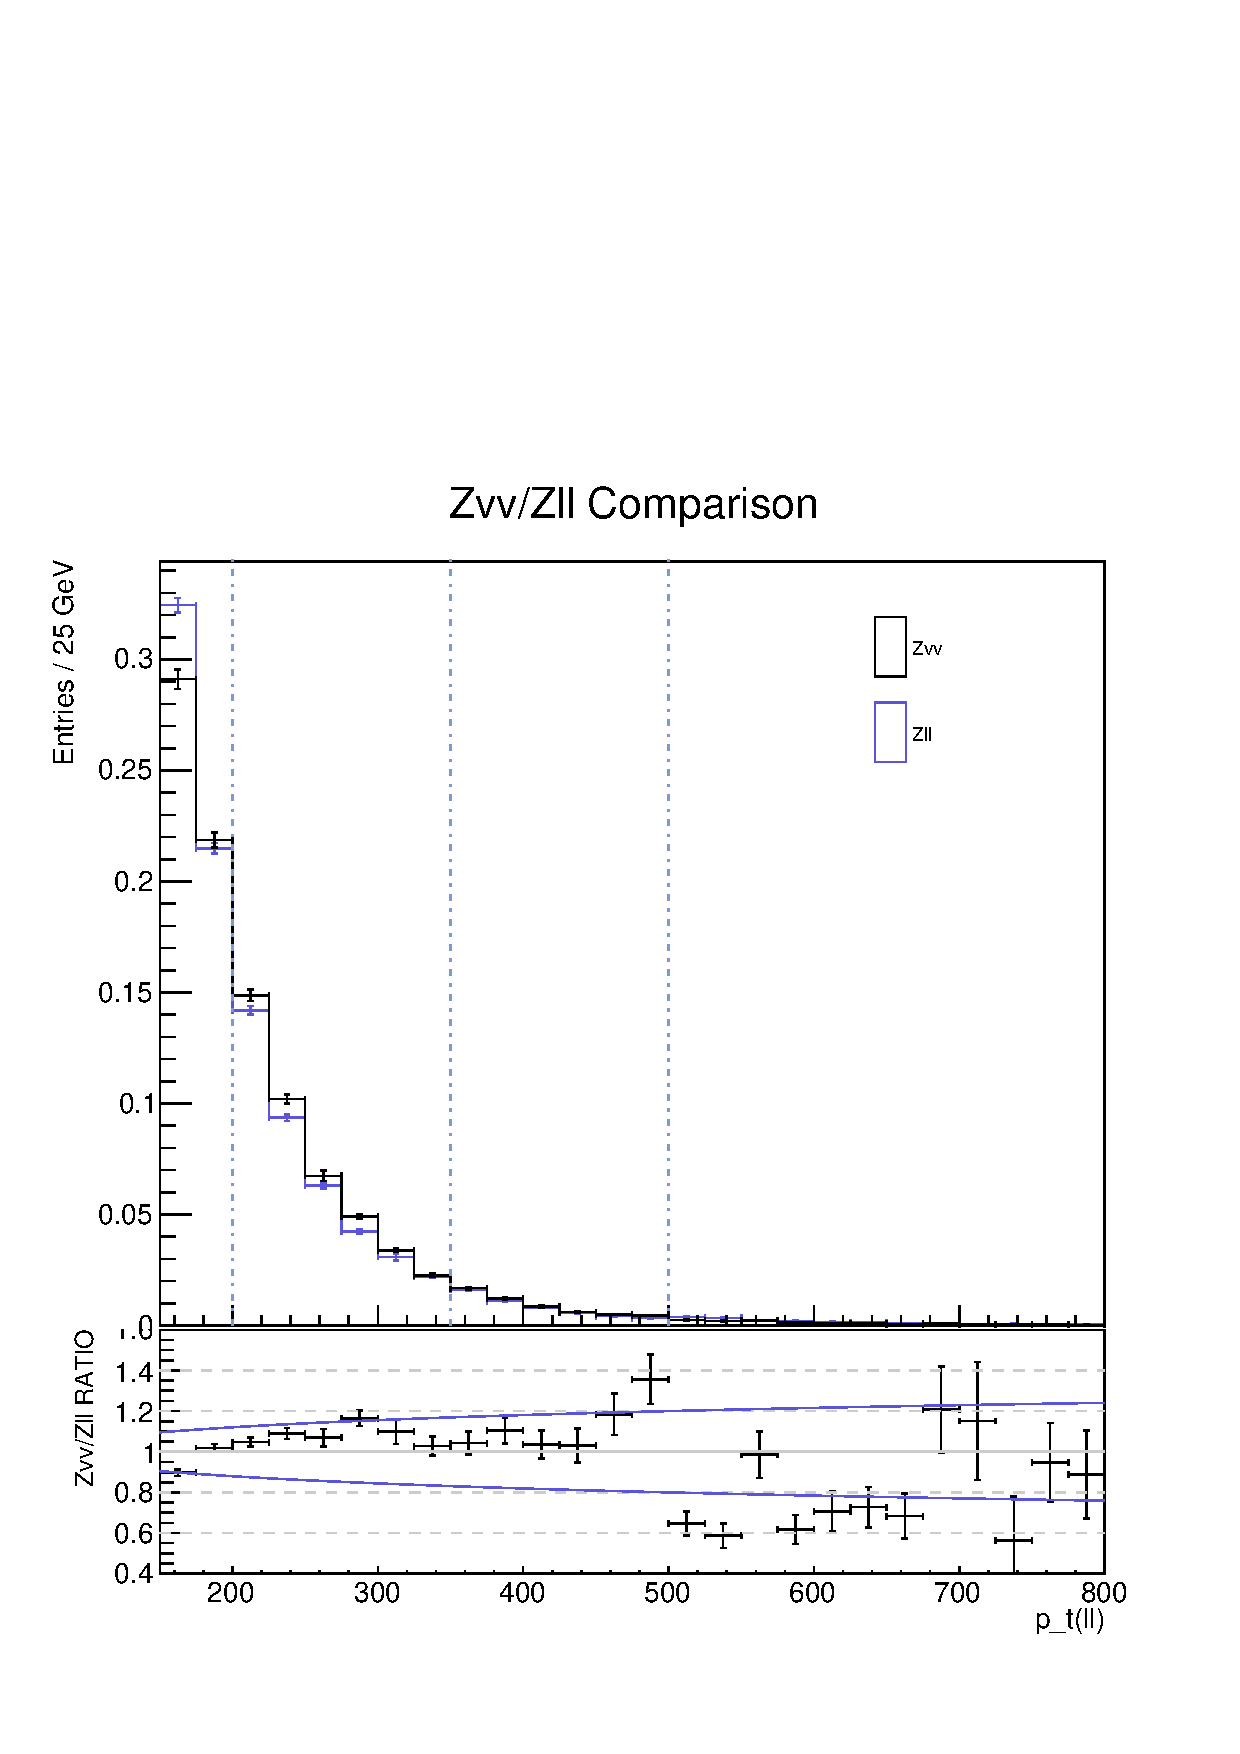
\includegraphics[width=0.45\linewidth]{twoMET.pdf}}
		%	\caption{\subref{fig:subfig_onePTV}The comparison of the (proxy) $E_T^{\mathrm{miss}}$ between SR and one-muon CR for the W($\mu \nu$)+jets events. \subref{fig:subfig_twoPTV}The compasion of the (proxy) $E_T^{\mathrm{miss}}$ between SR and two-lepton CR for the Z+jets events. Both the upper pannels show the normalized distribution and the lower pannels show the ratio of SR to CRs. The latter plot is meant to be an approximation to how large the ratio of the former plot is.}
		%	\label{fig:MET_comparison}
		%\end{figure}
	
		%\fig[0.5][fig:mjj_distribution][!hbt]{mjj_distribution.pdf}[The dijet mass distribution comparison of W($\mu \nu)$+jets in SR and one-muon CR. The upper pannel shows the distribution after normalization. The lower pannel shows the ratio of the yields in SR to one-muon CR.][short caption]
		
		From figure \ref{fig:MET_comparison}, two interseting things are found. First, the shape distribution has the same trend. Second, the ratios between the SR and one-muon CR are generally away from the 5\% difference as shown.  It is noticed that at lower energy, the ratios are larger than the upper limit and, at higher energy, the ratios are less than the lower limit, except for the last few bins, where the statistics are low. That is to say, at lower energy, W($\mu \nu$)+jets events underestimate the backgrounds in SR, and at higher energy, overestimation happens.
		
		In author's opinion, although the W($\mu \nu$)+jets events are the same in both SR and one-muon CR, the situation is a little bit different. These events would appear in the SR only when the muon is misidentified. If the muon is soft, which means it has low $p_T$, it's more likely to be misidentified and thus be reconstructed as $E_T^{\mathrm{miss}}$. On the other hand, if the $p_T$ is higher, misidentification are less likely to happen and the muon are rejected by the selection of SR. Therefore, more events whose muons have higher $p_T$ are removed in the SR but events with more low $p_T$ muons stay in the SR. This means that the true simulation, which is expected in one-muon CR, underestimates the yields at lower energy and overestimate at higher energy. Due to this poor estimation, one sees the severely flucuating ratio values.
		
		As a minor conclusion, the W($\mu \nu$)+jets comparison between SR and CR doesn't quite fit in the 5\% limit. One of the assumption on this is that the over- and under- estimation on different value of $p_T$ are not well covered by the uncertainty. The yield uncertainty shall be recalculated for this issue.

\chapter{Results of monoHbb Analysis}

\section{Main Uncertainties}
	The systematic uncertainties dominate the main uncertainty in this analysis. Among them, the b-tagging efficiency, the integrated luminosity, jet energy scale (JES) and jet energy resolution (JER) contribute the most to the experimental uncertainty. The SM predictions are the sources of the theoretical uncertainties. $t\bar{t}$ events, W/Z +jets events, associated production of SM Higgs boson decay into $b\bar{b}$ (Vh($b\bar{b}$), where V is the vector boson) and diboson events dominate the theoretical uncertainties.
	
	The uncertainty on the b-tagging efficiency originate from the flavor tagging efficiency in the $t\bar{t}$ events. A calibration, which highly makes use of beam testing in LHC, on the integrated luminosity is performed with a value a 2.0\%.
	
	The theoretical uncertainties originate from the SM modeling. Normalizations, acceptance difference and differential distributions of important kinematic variables derive the uncertainties.
	
\section{Results}
	A fit to the invariant mass of Higgs candidate $m_h$ is used to search for the signal. For resolved region, $m_{\mathrm{jj}}$ represents the Higgs mass while $m_{\mathrm{J}}$ is used in the merged region.
	
	The fit is based on a likelihood based approach. The systematic uncertainties are used in the likelihood function as nuisance parameters. The data in SR and two CRs are fit simultaneously for all four different (proxy) $E_T^{\mathrm{miss}}$ bins: $\left[150, 200\right)$ GeV, $\left[200, 350\right)$ GeV, $\left[350, 500\right)$ GeV, and $\left[500, \infty \right)$ GeV. $m_h$ is the fit variable in the SR. The fit variable used in the one-muon CR is the $\mu$ lepton charge. $t\bar{t}$ processes tend to produce the same amount of $\mu^+$ and $\mu^-$ leptons but the W+jets events produce more $\mu^+$ than $\mu^-$ leptons, which originates from proton-proton collision in LHC and from the conservation of electric charge. $\mu$-charge can thus be made use of as a differentiation of $t\bar{t}$ and W+jets events. In the two-lepton CR, the event yields serve as the fit variable because of limited data statistics.
	
	Figure \ref{fig:MET_SR} shows the $E_T^{\mathrm{miss}}$ distribution in SR. Figure \ref{fig:SR_mj} shows the distribution of $m_{\mathrm{jj}}$ or $m_{\mathrm{J}}$ in SR for resolved and merged region respectively. The data yields agree with the SM predictions. That is to say, no significant excess of the signal is found.
	
	An exclusion limit at 95\% confidence level (CL) is used for the interpretation of this analysis. The exclusion contour in $(m_{\mathrm{A}}, m_{\mathrm{Z'}})$ phase space is shown in figure \ref{fig:exclusion}. It also shows the result in the previous iteration. As it suggests, more region are excluded compared to the previous result. Figure \ref{fig:signal strength} shows the comparison of the upper limit of the signal strength between this result and the previous result, in which the fixed-radius (FR) track jets are used. In contrast to VR, FR track jets have a fixed cone size of $R = 0.2$. The plot also suggests more region in the phase space is excluded.
	
	\fig[0.6][fig:MET_SR][!hbt]{MET_SR.png}[The $E_T^{\mathrm{miss}}$ distribution for resolved and merged combined in SR. The dashed blue lines are the expectation yields before fits. The solid histograms are the simulations after fit. The dashed red lines are the expected signal from Z'-2HDM model.][short caption]
	
	\begin{figure}[!hbt]
		%\captionsetup[subfigure]{labelformat=empty} % hide figure's number.
		\centering
		\subcaptionbox
		{\label{fig:subfig_SR_mjj_150_200}}
		{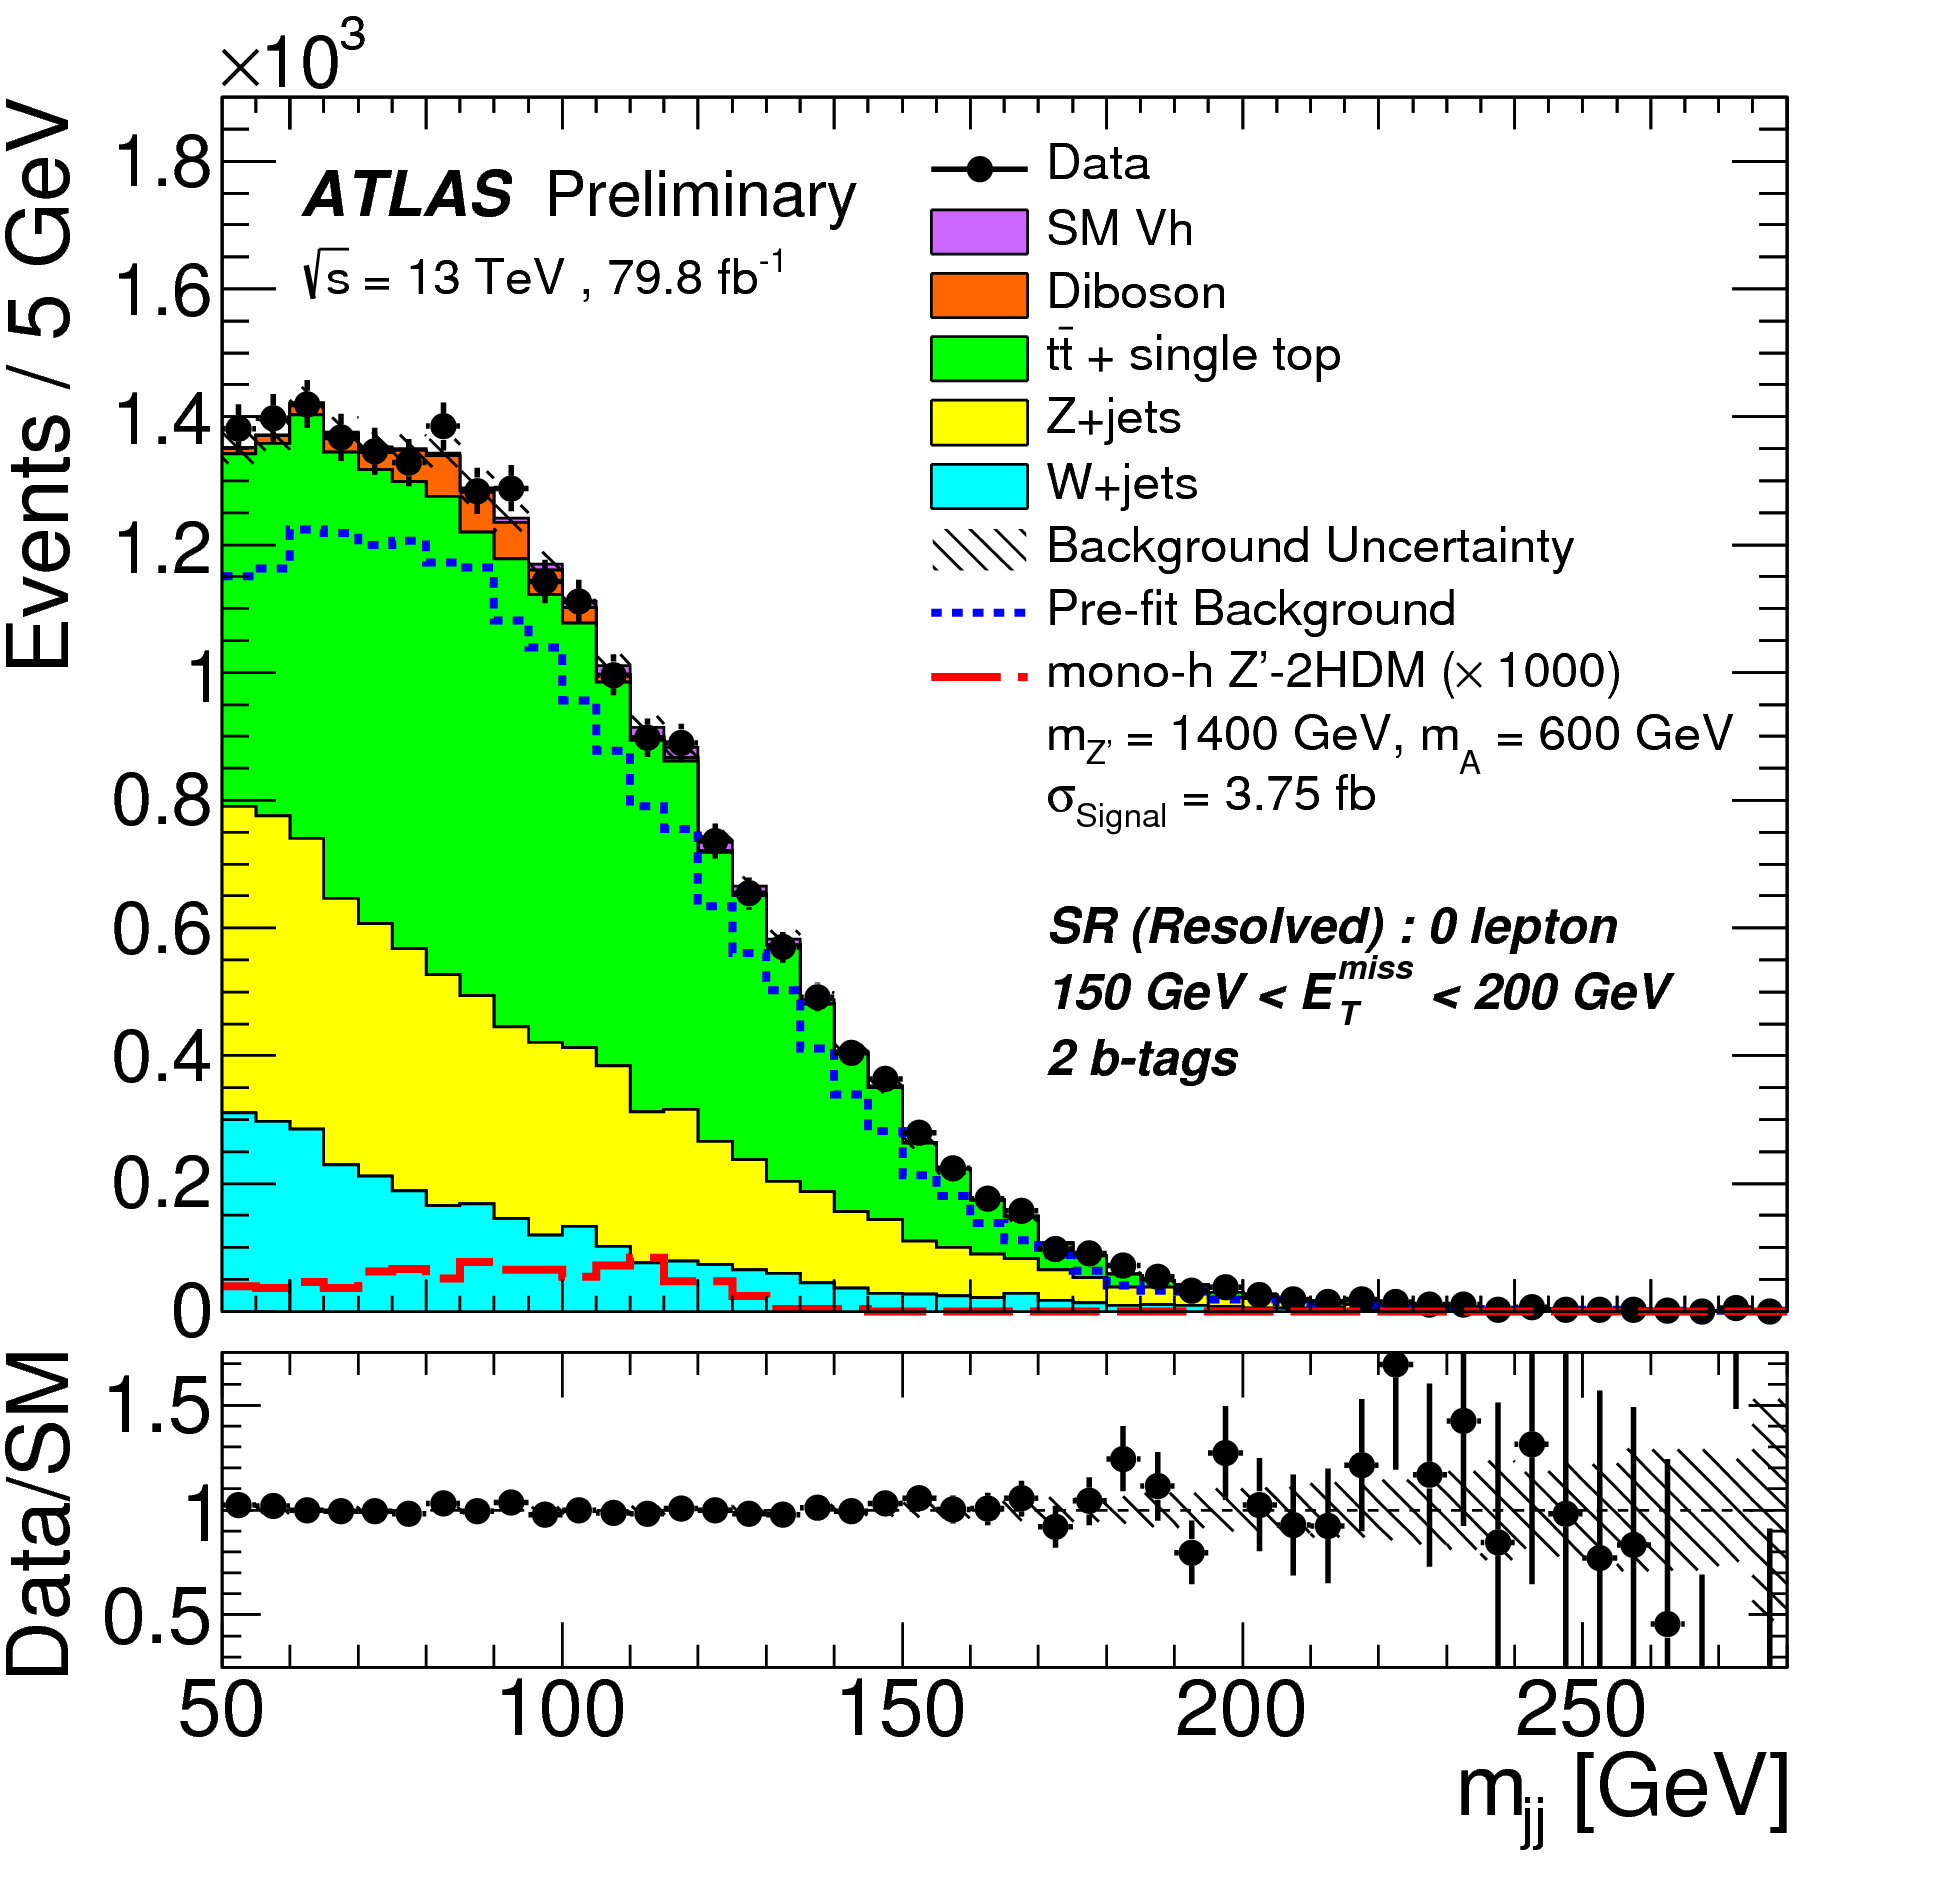
\includegraphics[width=0.4\linewidth]{SR_mjj_150_200.png}}
		~
		\subcaptionbox
		{\label{fig:subfig_SR_mjj_200_350}}
		{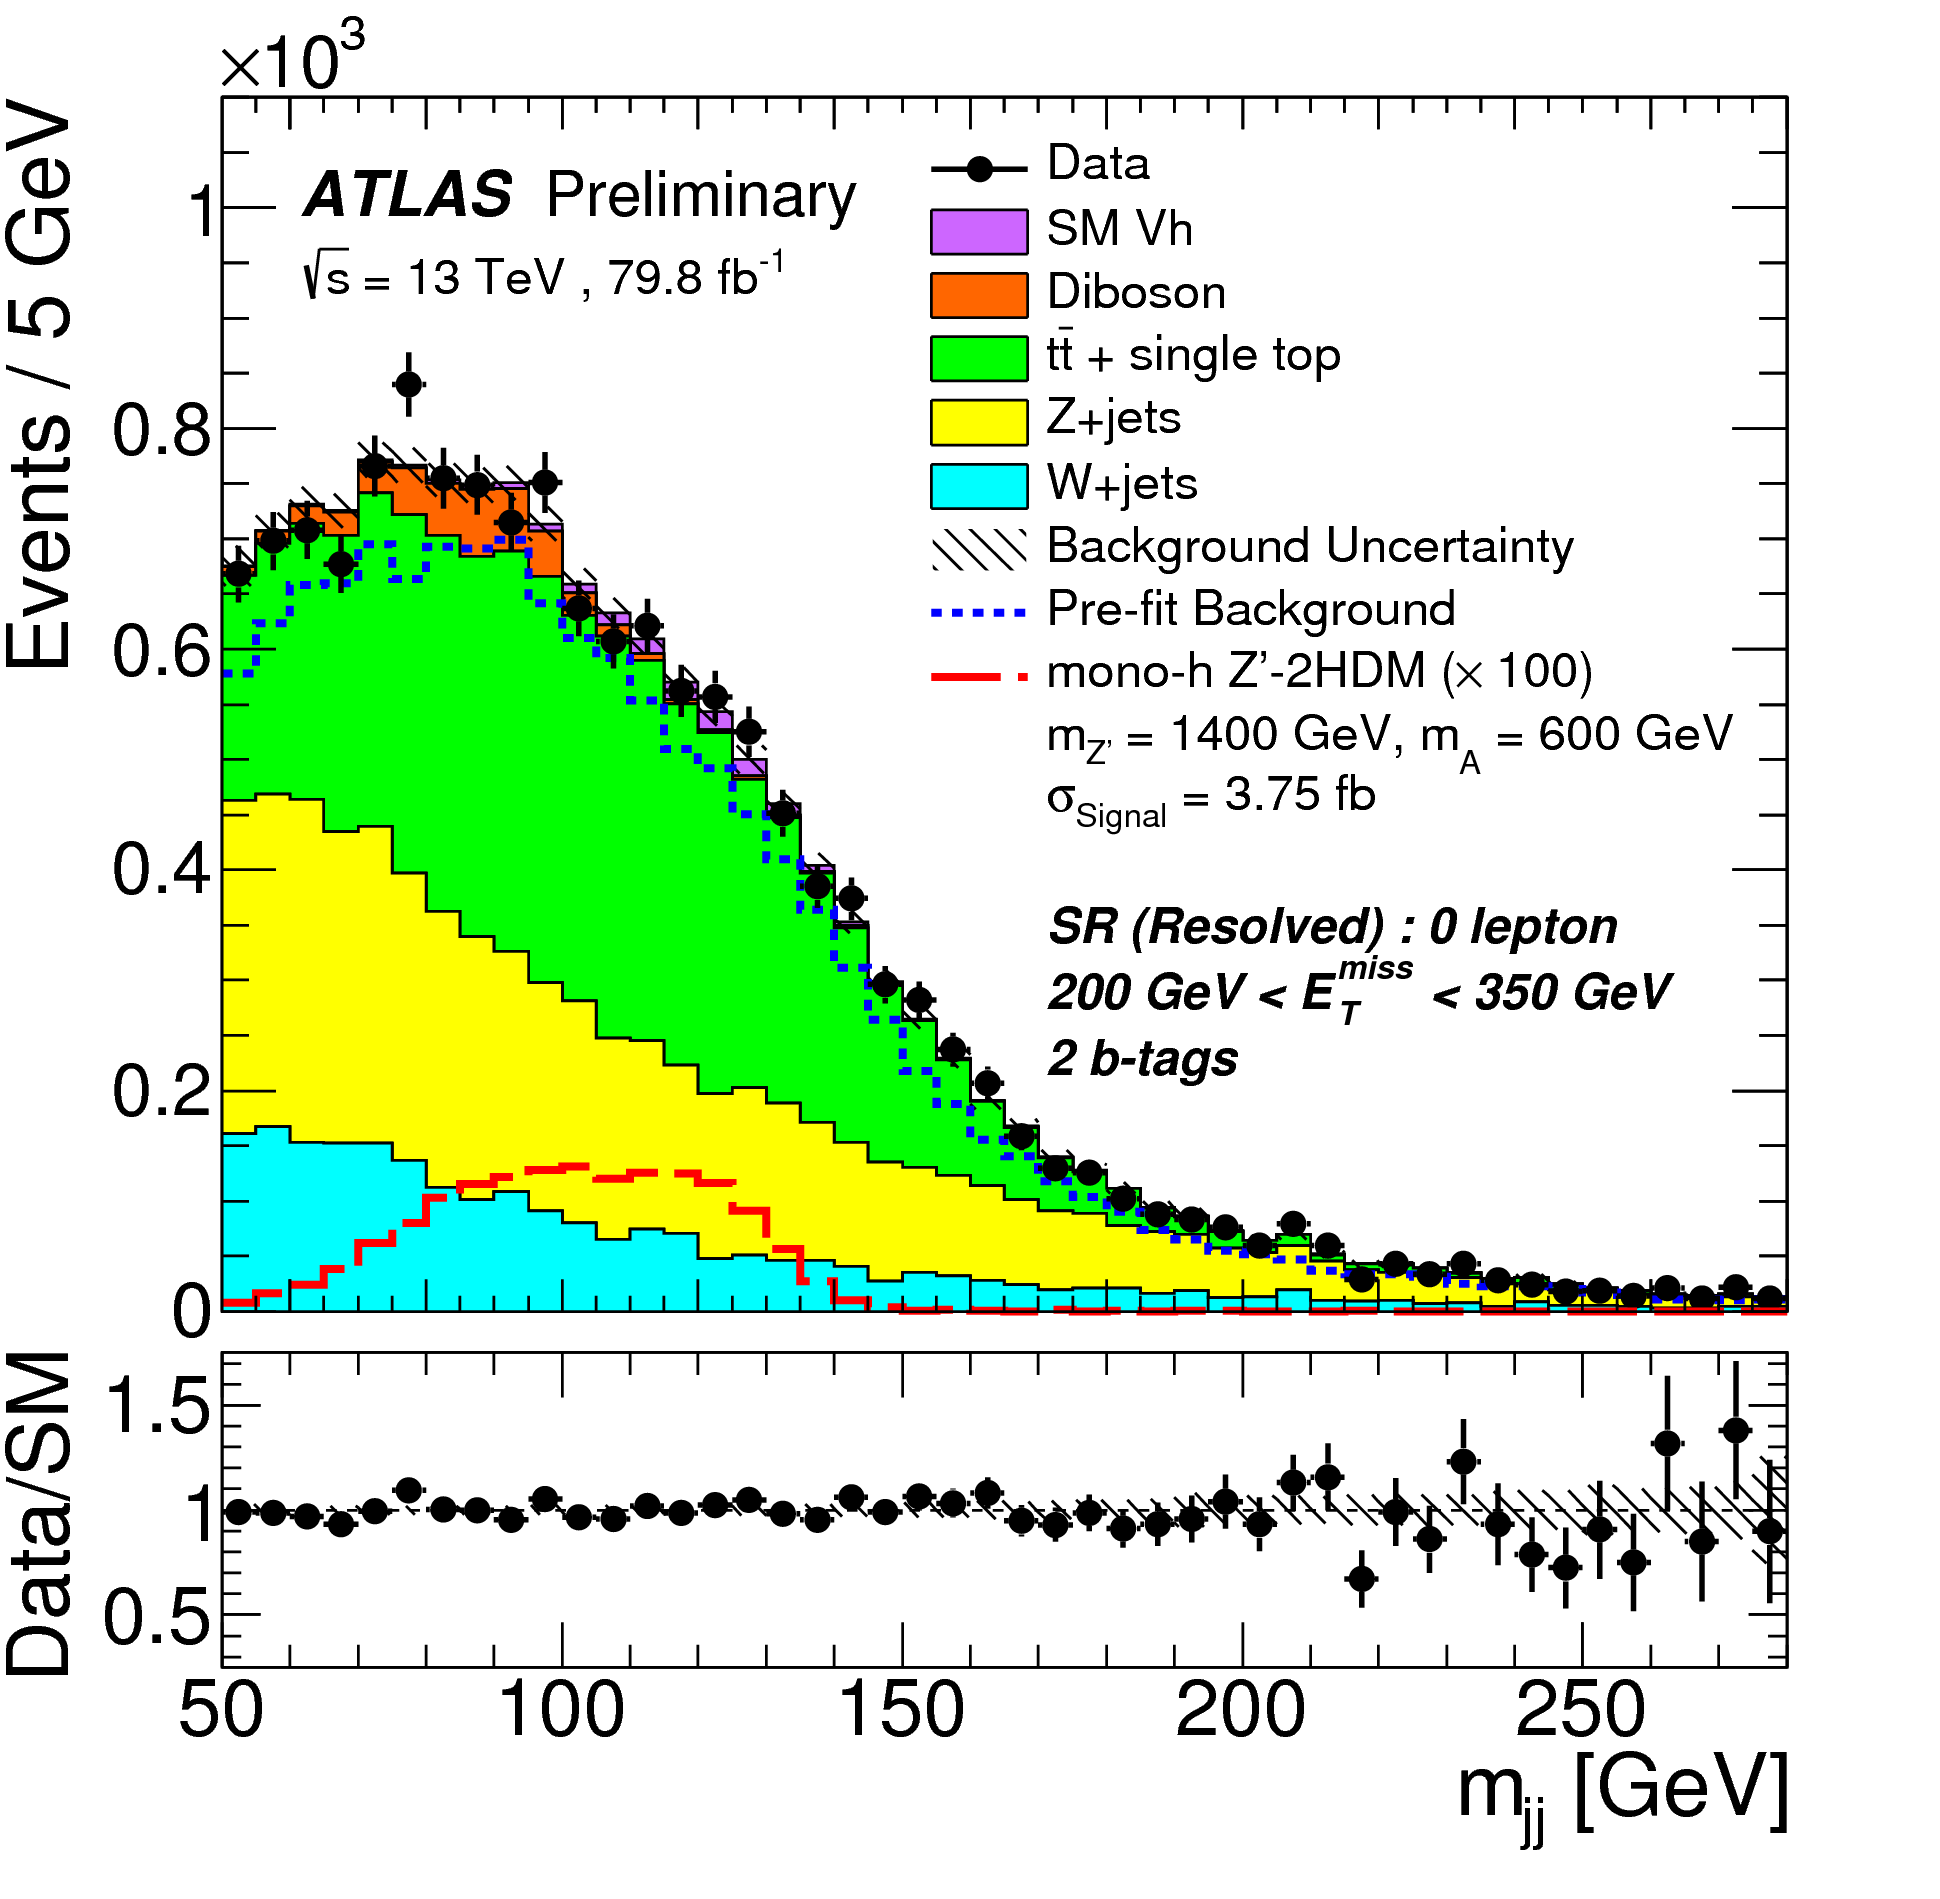
\includegraphics[width=0.4\linewidth]{SR_mjj_200_350.png}}
		\vspace{\baselineskip} % 分隔上下列
		\subcaptionbox
		{\label{fig:subfig_SR_mjj_350_500}}
		{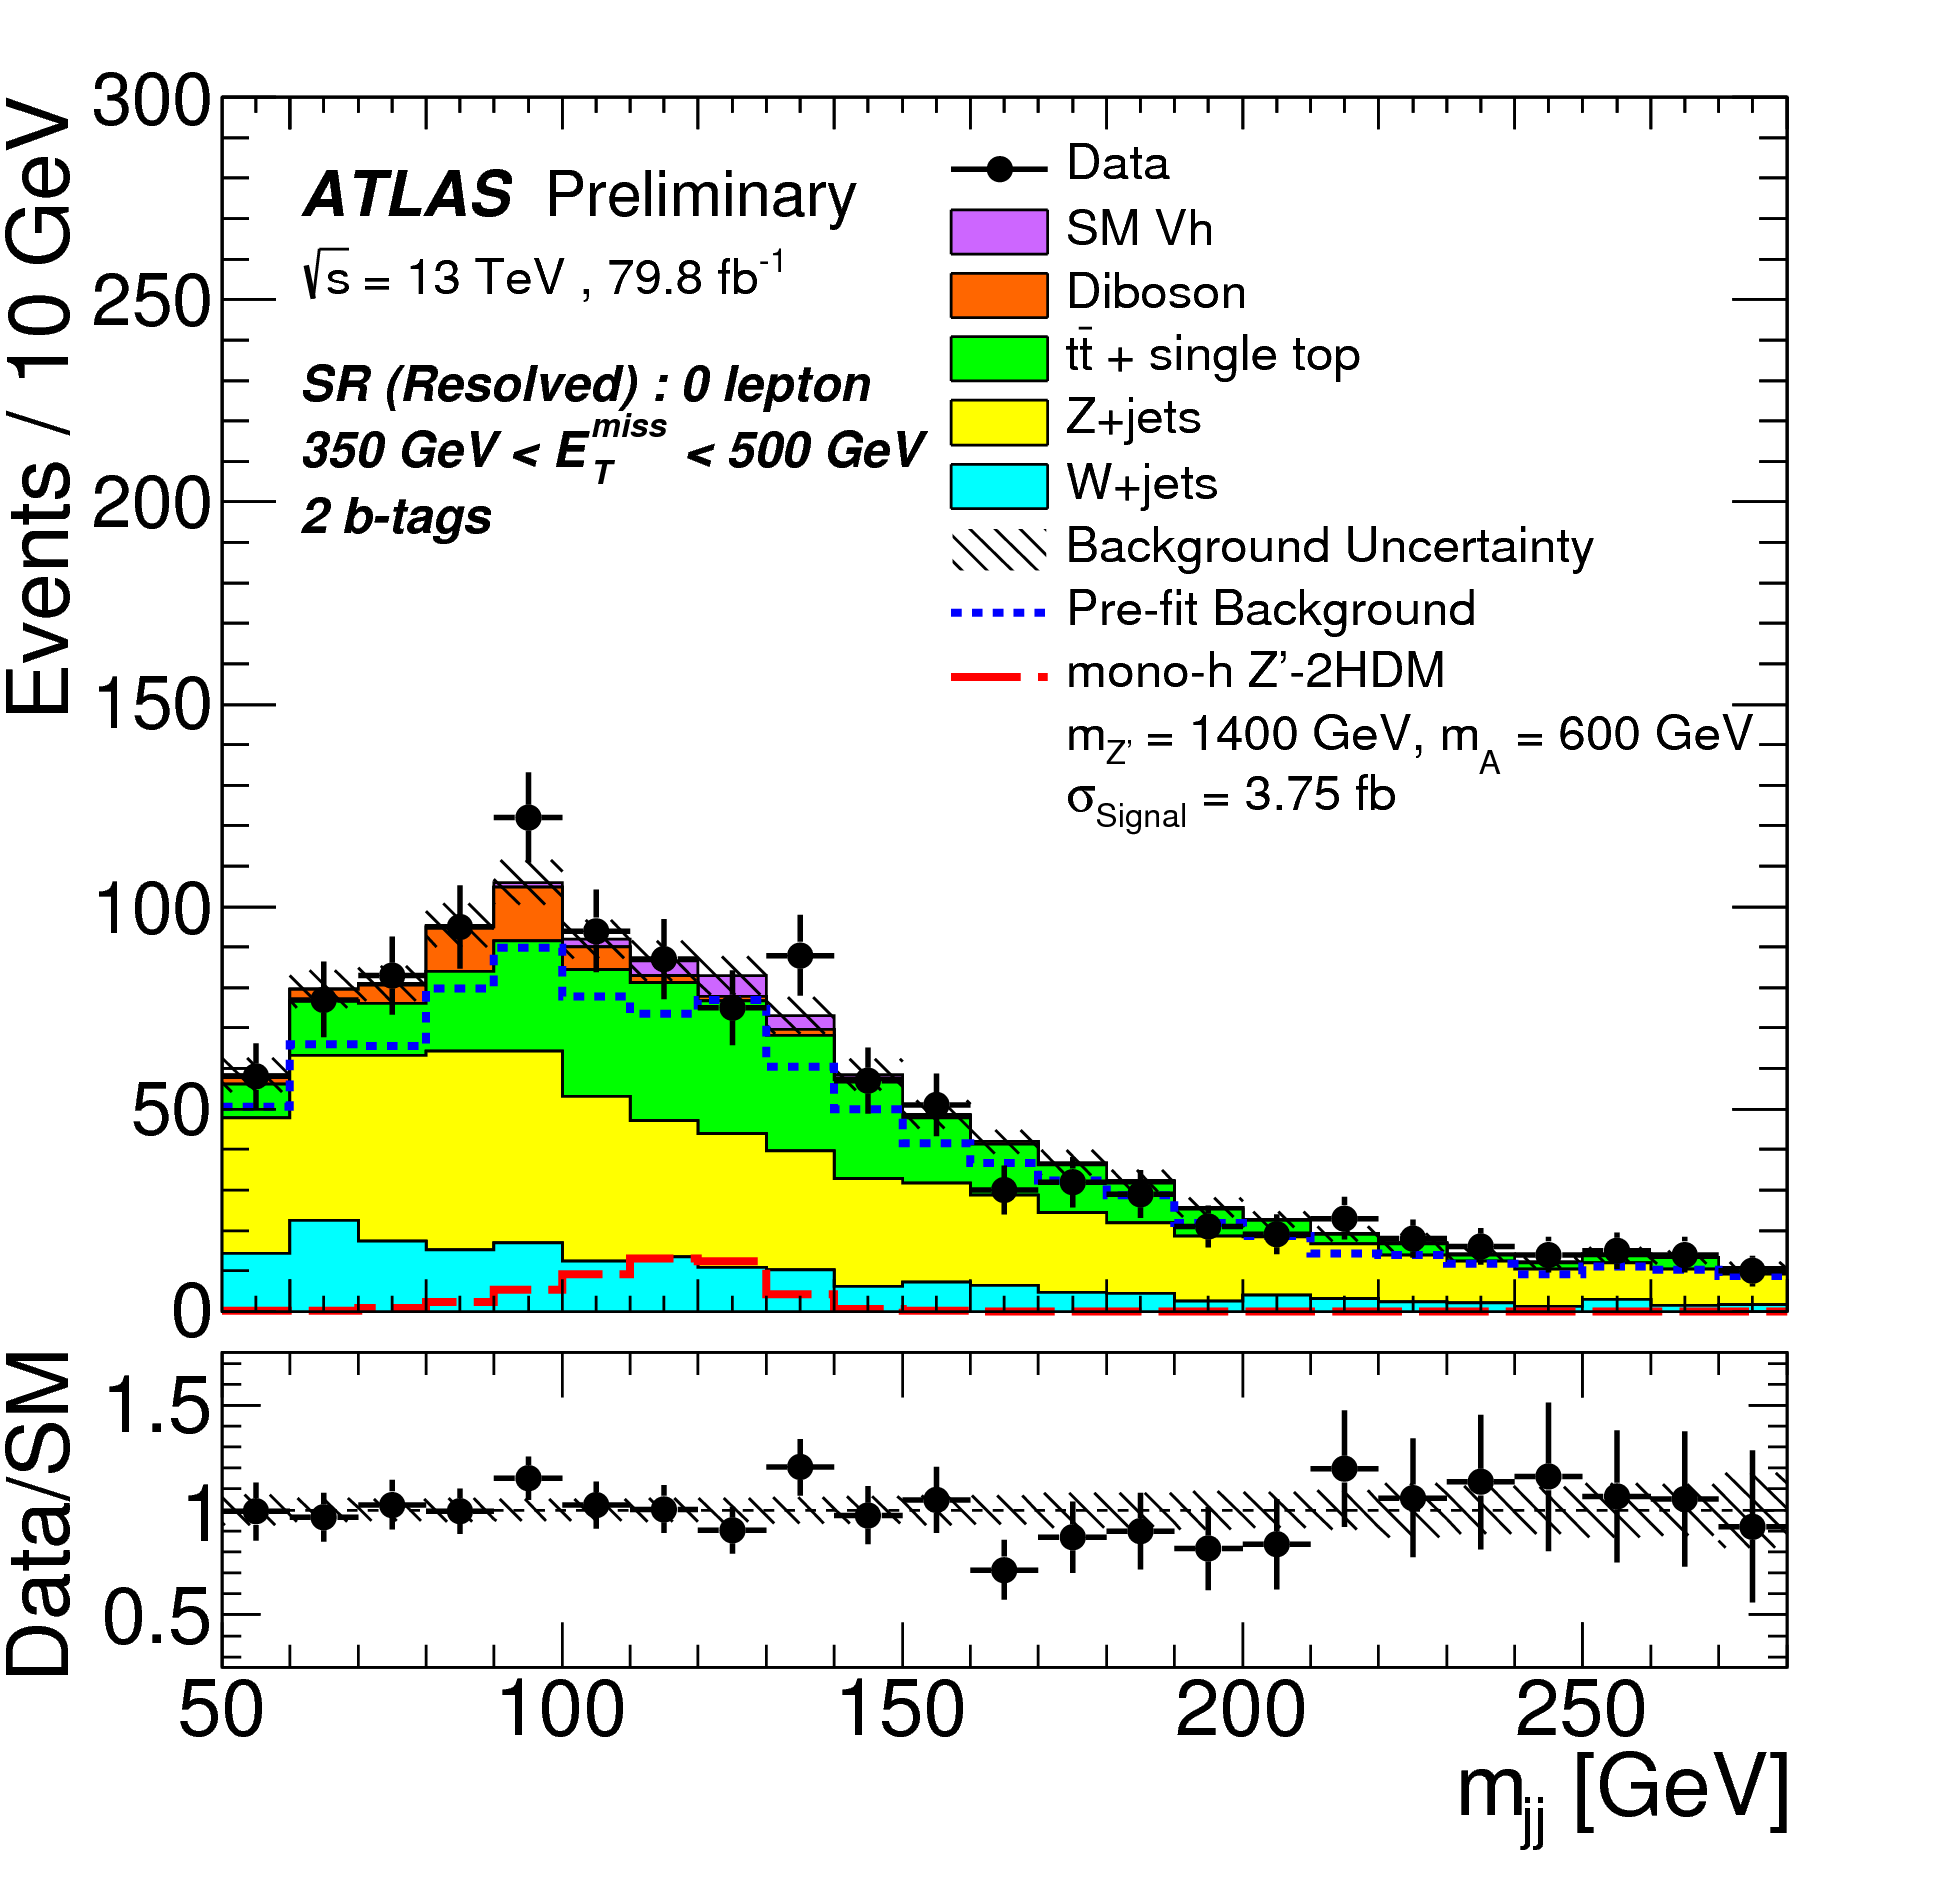
\includegraphics[width=0.4\linewidth]{SR_mjj_350_500.png}}
		\subcaptionbox
		{\label{fig:subfig_SR_mJ_500}}
		{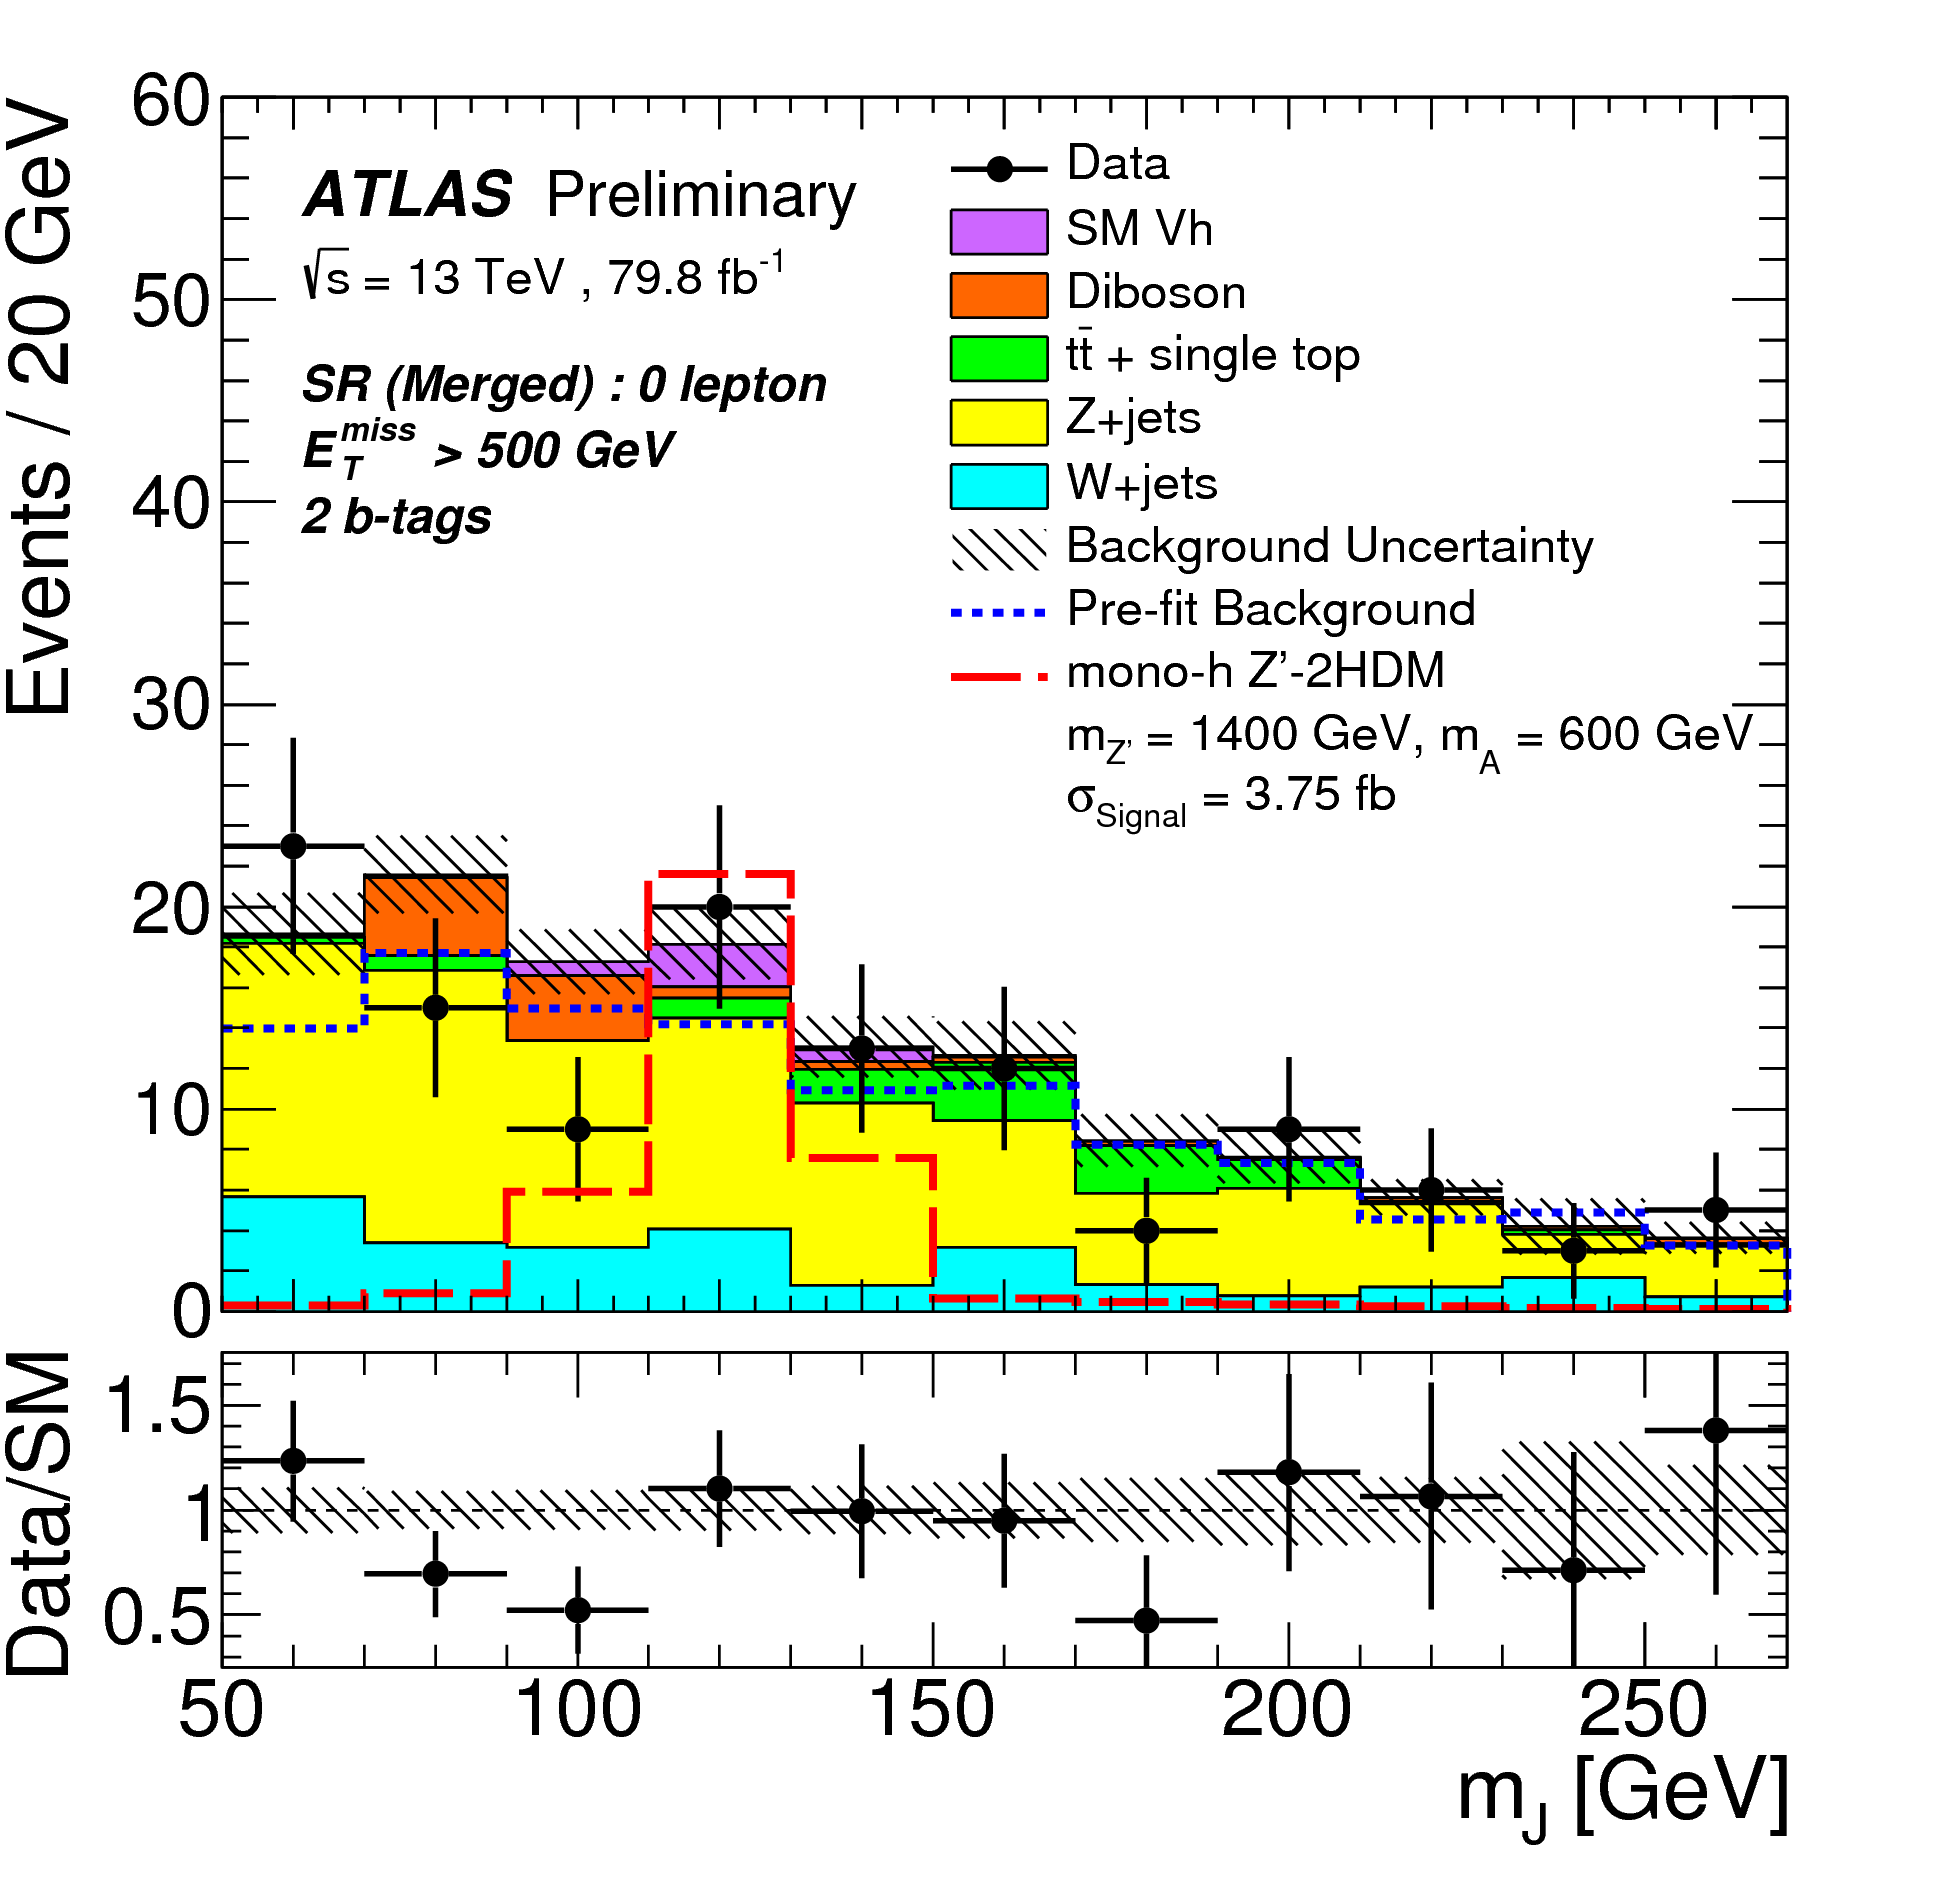
\includegraphics[width=0.4\linewidth]{SR_mJ_500.png}}
		\caption{Distirbution of the invariant mass of the Higgs boson candidate $m_{\mathrm{h}}$ with two b-tagged jets. The upper two plots are for $E_T^{\mathrm{miss}} \in \left[150, 200\right)$ GeV and $\left[200, 350\right)$ GeV bins. The lower two ones are for $E_T^{\mathrm{miss}} \in \left[350, 500\right)$ GeV and $\left[500, \infty \right)$ GeV. The dashed blue lines are the expectation yields before fits. The solid histograms are the simulations after fits. The dashed red lines are the expected signal from Z'-2HDM model. Its yields for the upper two plots are scaled up by a factor of 100 and 1000 from left to right respectively.}
		\label{fig:SR_mj}
	\end{figure}
	
	\fig[0.6][fig:exclusion][!hbt]{exclusion.png}[Exclusion contour in $(m_{\mathrm{A}}, m_{\mathrm{Z'}})$ phase space. Regions under the curve are excluded. The solid line shows consistency with SM-only hypothesis. The dashed blue line are the results from previous ATLAS results of $\sqrt{s} = 13$ TeV.][short caption]
	
	\fig[0.6][fig:signal strength][!hbt]{signal_strength.png}[The upper limit of the signal strength of this model with $m_{\mathrm{A}}$ fixed at 500 GeV. The dashed red line is the result of previous iteration, which made use of FR track jets. The dashed black line in the result of this iteration, where VR track jets are used. Signals, if exist, would appear in the region where the signal strength is greater than one. As a result, all regions whose upper limit is smaller than one is excluded. As the plot shows, making use of VR track jets extends the excluded region.][short caption]


\chapter{Conclusion}\label{result}
	To sum up, a collider search for the dark matter in association with a final state of $E_T^{\mathrm{miss}}$ and $b\bar{b}$, which decay from the Higgs boson candidate, was performed using 79.8 $fb^{-1}$ of proton-proton collision at $\sqrt{s} = 13$ TeV recorded in the ATLAS at LHC. The results are in agreement with SM predictions. An exclusion on the parameter space of Z'-2HDM model is excluded, up to $m_{\mathrm{Z'}} = 2.8$ TeV and $m_{\mathrm{A}} = 300$ GeV.


\chapter{Reference}

\end{document}